
\documentclass{beamer}
\usetheme{boxes}
\setbeamerfont*{frametitle}{size=\normalsize,series=\bfseries}
\setbeamertemplate{navigation symbols}{}
\setbeamercolor{block body}{fg=black!75!blue!85!white}
\useoutertheme{infolines}
\setbeamertemplate{headline}{} % removes the headline that infolines inserts

\usepackage[english]{babel}
\usepackage[latin1]{inputenc}
\usepackage{times}
\usepackage[T1]{fontenc}
\usepackage{mathbbol}

\usepackage{amsthm}
\usepackage[font=scriptsize,labelfont=bf]{caption}

\title[3D Model of the genome]
{%
Structure estimation for discrete graphical models - Generalized covariance
matrices and their inverses
}

\author[Varoquaux]
{
  Nelle~Varoquaux\inst{1}
}

\institute[Mines ParisTech]
{
  \inst{1}%
  Mines ParisTech
}

\begin{document}


\begin{frame}
  \maketitle
\end{frame}

\begin{frame}
\frametitle{Graphical models}
\begin{itemize}
\item An undirected graph $G = (V, E)$ consists of a collection of $p$
vertices $ V = \{1, 2, \dots, p \}$ and a collection of unordered vertex pairs
$E \subseteq V \times V$
\item To each vertex $s \in V$ is associated a random variable $X_s$ taking
values in some space $\mathcal{X}$.
\item Let $C \subseteq V$ be a clique and $\mathcal{C}$ the ensemble of
cliques.
\item The distribution of $X$ can be factorized:
\begin{equation}
\mathbb{P}_\theta(x_1, \dots, x_p) \propto exp(\{ \sum_{C \in \mathcal{C}}
\theta_C (x_C) \mathbb{1}_C(x_C) - \Phi(\theta) \})
\end{equation}
\end{itemize}
\end{frame}

\begin{frame}
\frametitle{Relationship between the covariance matrix and the graph
structure}
\begin{itemize}
\item Let $\Sigma = \text{cov} (X_1, \dots, X_2)$ be the covariance matrix.
\item Let $\Gamma = \Sigma ^{-1}$ be its inverse.
\end{itemize}

\vspace{10px}
{\small
\begin{block}{Consequence of the Hammersley-Clifford theorem on Gaussian
Graphical Models}
\begin{itemize}
\item $\Gamma_{st}$ is the magnitude of the correlation of $X_s$ and $X_t$
conditionned on $X_{\{s,t\}}$.
\item The sparsity of $\Gamma$ reflects the graph structure.
\end{itemize}
\end{block}
\vspace{10px}
}
\textcolor{black!35!red}{To which measure can this be extended to discrete graphical
models?}

\end{frame}


\begin{frame}
\frametitle{Covariance matrices on examples}

\begin{columns}
\begin{column}{0.5\textwidth}
\begin{figure}
\includegraphics[width=65px]{./images/chain.png}
\includegraphics[width=65px]{./images/dino.png}
\end{figure}

\end{column}

\begin{column}{0.5\textwidth}
\begin{figure}
\includegraphics[width=65px]{./images/loop.png}
\includegraphics[width=65px]{./images/loop_augmented.png}
\end{figure}

\end{column}
\end{columns}

\begin{overlayarea}{10cm}{1.2cm}
\only<1>{
\begin{block}{Inverse covariance of a chain {\small \textcolor{black!75!blue}{($\theta_{s} = 0.1$, $\theta_{s,
t} = 2$)}}}
\end{block}
}

\only<2>{
\begin{block}{Inverse covariance of a loop}
\end{block}
}

\only<3>{
\begin{block}{Inverse augmented covariance of a chain {\tiny \textcolor{black!75!blue}{$(X_1, X_2, X_3, X_4, X_1X_3)$}}}
\end{block}
}
\end{overlayarea}

\begin{overlayarea}{10cm}{5cm}

\begin{center}
\only<1>{
{\small
$\Gamma_{\text{chain}} = 
\begin{bmatrix}
9.80 & -3.59 & 0 & 0 \\
-3.59 & 34.30 & -4.77 & 0 \\
0 & -4.77 & 34.30 & -3.59 \\
0 & 0 & -3.59 & 9.80 \\
\end{bmatrix}$
}}


\only<2>{
{\small
$\Gamma_{\text{loop}} = 
\begin{bmatrix}
51.37 & -5.37 & -0.17 & -5.37 \\
-5.37 & 51.37 & -5.37 & -0.17 \\
-0.17 & -5.37 & 51.37 & -5.37 \\
-5.37 & -0.17 & -5.37 & 51.37 \\
\end{bmatrix}$}}

\only<3>{
{\small
$\Gamma_{\text{augmented}} = 10 ^3 \times
\begin{bmatrix}
1.15 & -.0.2 & 1.09 & -0.02 & -1.14 \\
-0.02 & 0.05 & -0.02 & 0 & 0.01 \\
-0.02 & 0 & -0.02 & 0.05 & 0.01 \\
-1.14 & 0.01 & -1.14 & 0.01 & 1.19 \\
\end{bmatrix}
$}}
\end{center}
\end{overlayarea}

\end{frame}

\begin{frame}
\frametitle{Triangulation}

\begin{figure}
\begin{center}
\includegraphics[width=50px]{./images/loop.png}
\includegraphics[width=50px]{./images/loop_augmented.png}
\end{center}
\end{figure}

\begin{definition}
Given an undirected graph $G = (V, E)$, a triangulation is an augmented graph
$\hat{G} = (G, \hat{E})$ that contains no chordless cycles of length 4.
\end{definition}
\end{frame}

\begin{frame}
\frametitle{Triangulation and block-graph-structure}

\begin{theorem}
Consider an  arbitrary discrete graphical model of the form (4), and let
$\mathcal{T}$ be the set of maximal cliques in any triangulation of $G$. Then,
the inverse $\Gamma$ of the augmented covariance matrix is block
graph-structured.
\begin{itemize}
\item For any two subset $A, B \in \hat{\mathcal{C}}$ that are not subsets of
the same maximale cliques, the block $\Gamma(A, B)$ is identically zero.
\item For almost all parameters $\theta$, the entire block $\Gamma(A, B)$
nonzero whenever $A$ and $B$ belong to a common maximal clique.
\end{itemize}
\end{theorem}
\end{frame}

\begin{frame}
\frametitle{Consequences}
\begin{itemize}
\item A tree or a dino graph is already triangulated. $\Gamma$ reflects the
graph structure.
\item When a graph $G$ is not triangulated, we may need to invert a larger
augmented covariance matrix.
\end{itemize}
\end{frame}

\begin{frame}
\frametitle{Algorithm}

\begin{enumerate}
\item Form a suitable estimate $\hat{\Sigma}$ of the true covariance matrix
$\Sigma$
\item Optimize the graphical Lasso program with parameter $\lambda_n$,
denoting the solution by $\hat{\Theta}$
\item Threshold the entries of $\hat{\Theta}$ at level $\theta_n$ to obtain an
estimate of $\Theta^*$
\end{enumerate}

\begin{columns}
\begin{column}{0.5 \textwidth}
\begin{equation*}
\lambda_n \geq \frac{c_1}{\alpha} \sqrt{\frac{\log p}{n}}
\end{equation*}
\end{column}
\begin{column}{0.5 \textwidth}
\end{column}

\begin{equation}
\end{equation}
\end{columns}

\end{frame}


\begin{frame}
\frametitle{Results}

\begin{figure}
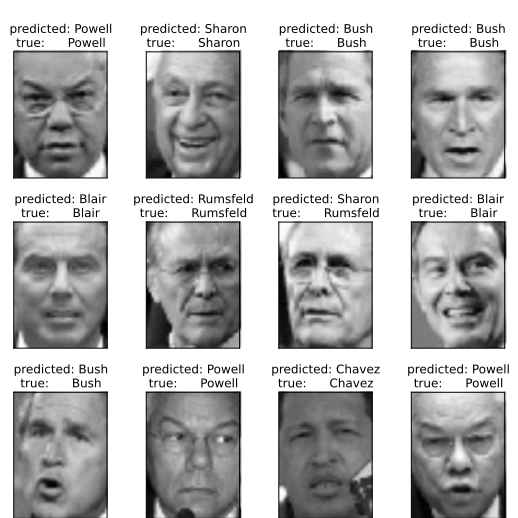
\includegraphics[width=300px]{./images/results.png}
\end{figure}
\end{frame}

\end{document}
